\documentclass[oneside, a4paper ,12pt]{book}
\usepackage[utf8]{inputenc}
\usepackage{graphicx}

\begin{document}

\author{Octavianus Immanuel Christpurwanto \\ 5024211014}
\title{Laporan Game \\ \emph{Escape The Labyrinth} \\ 
\includegraphics[width=8 cm]{screenshot001.png}}
\date{Desember 2022}

\frontmatter
\maketitle
\tableofcontents

\mainmatter
\chapter{Pendahuluan}
\section{Latar Belakang}

 \textit{Game} merupakan jenis hiburan yang pada zaman ini sering sekali digunakan banyak orang, mulai dari anak kecil hingga orang dewasa, untuk melepaskan rasa lelah setelah lama beraktivitas. Bukan hanya untuk melepas rasa lelah setelah beraktivitas, \textit{game} juga bisa digunakan untuk melatih pola pikir seseorang.
 
 Banyaknya game yang sudah berkembang saat ini tentunya membuat game itu memiliki setiap pengelompokkan berdasarkan \textit{gameplay} dari banyak game tersebut, yang biasa disebut \textit{genre game.}
 
 Pada perkuliahan Struktur Data dan Analisa Algoritma ini, kami para mahasiswa kelas A yang diajar oleh dosen Pak Eko Mulyanto diberi tugas \emph{final project} yaitu membuat \emph{game} yang kami buat sendiri dengan kemampuan yang kami bisa, baik menggunakan sfml di codeblock atau visual studio, bahkan tanpa menggunakan sfml. Akan tetapi, kami tidak dianjurkan menggunakan \emph{game engine} yang sudah ada seperti unity, unreal engine, dan lainnya, serta menggunakan bahasa C/C++.
 
 \section{Penjelasan Game}
 
 \emph{Game} yang saya buat adalah game \emph{Escape The Labyrinth} yang memiliki tujuan \emph{player} yang kita mainkan harus mencari pintu keluar yang ada di labirin tersebut, dengan adanya musuh dan jalan yang tentunya bercabang-cabang.
 
 \chapter{Desain}
 \section{Desain Game dan Karakter}
 \begin{figure} [h]
 		\centering
 		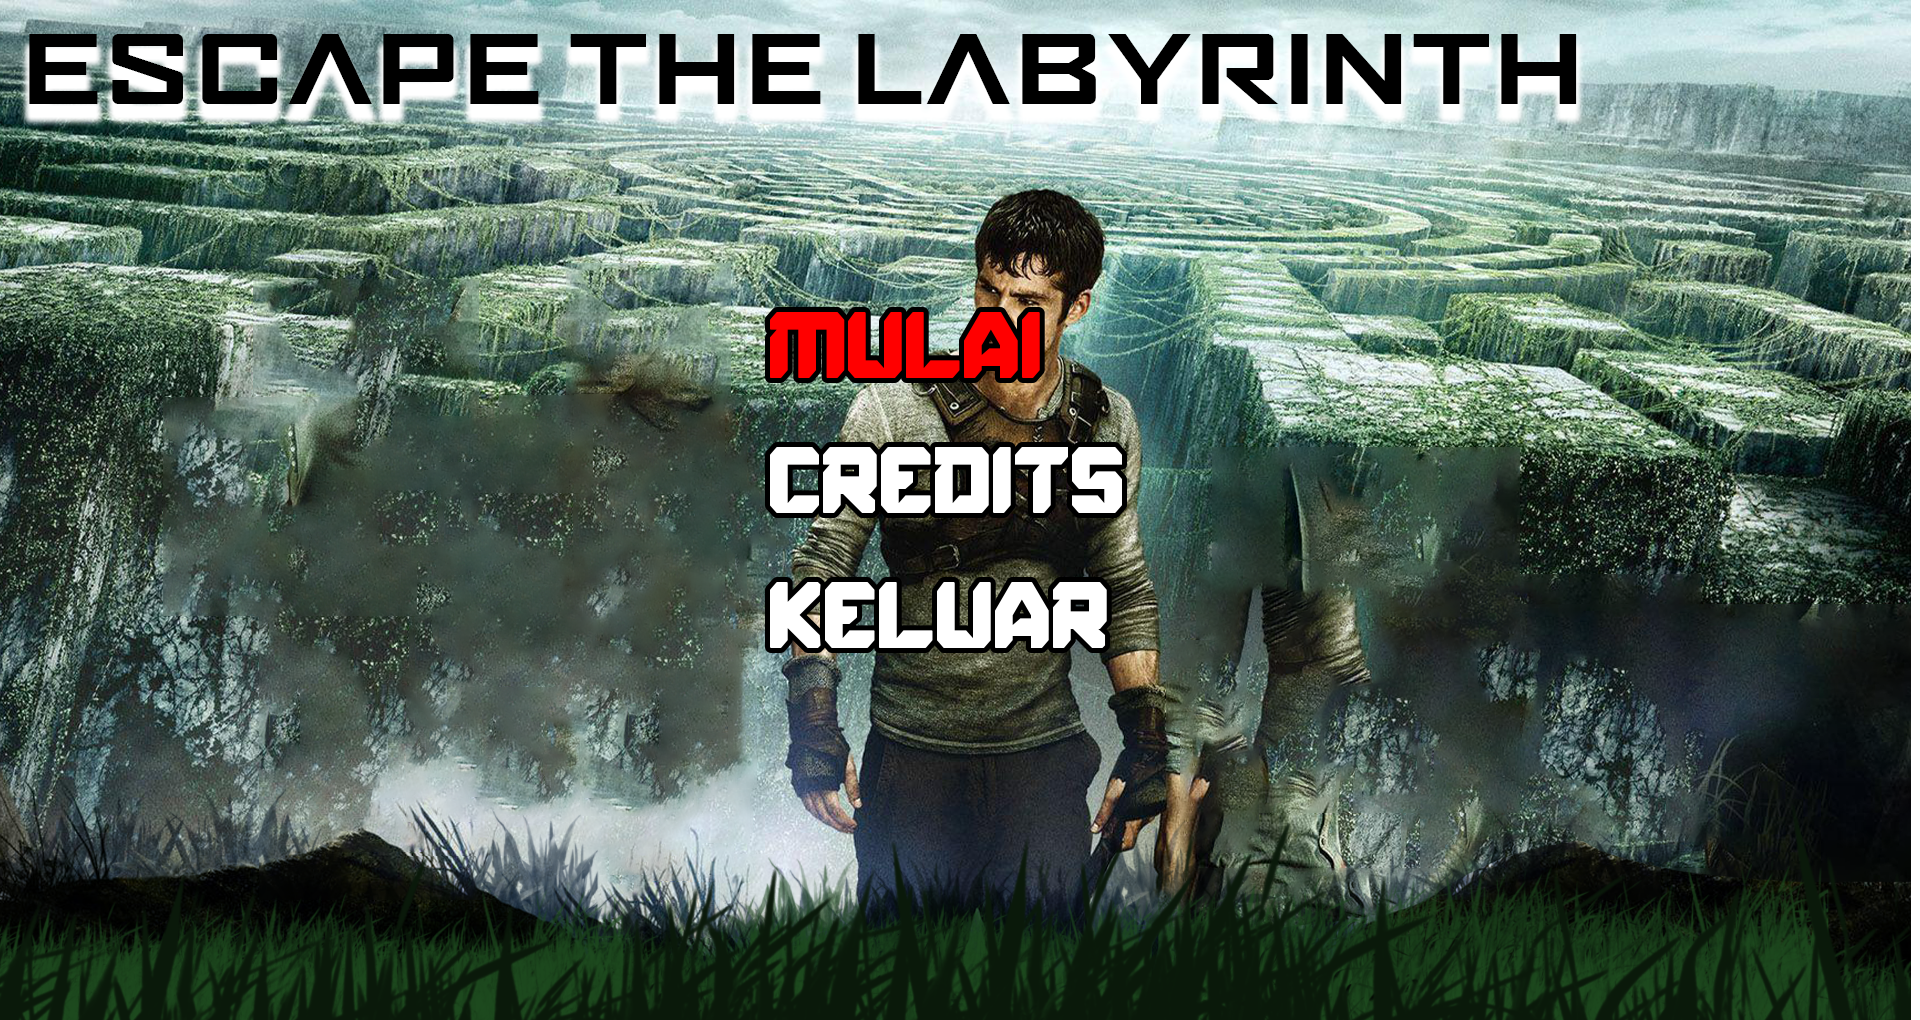
\includegraphics[width=10 cm]{Main Menu.png}
 		\caption{Main Menu}
 \end{figure}
 \begin{figure} [h]
 		\centering
 		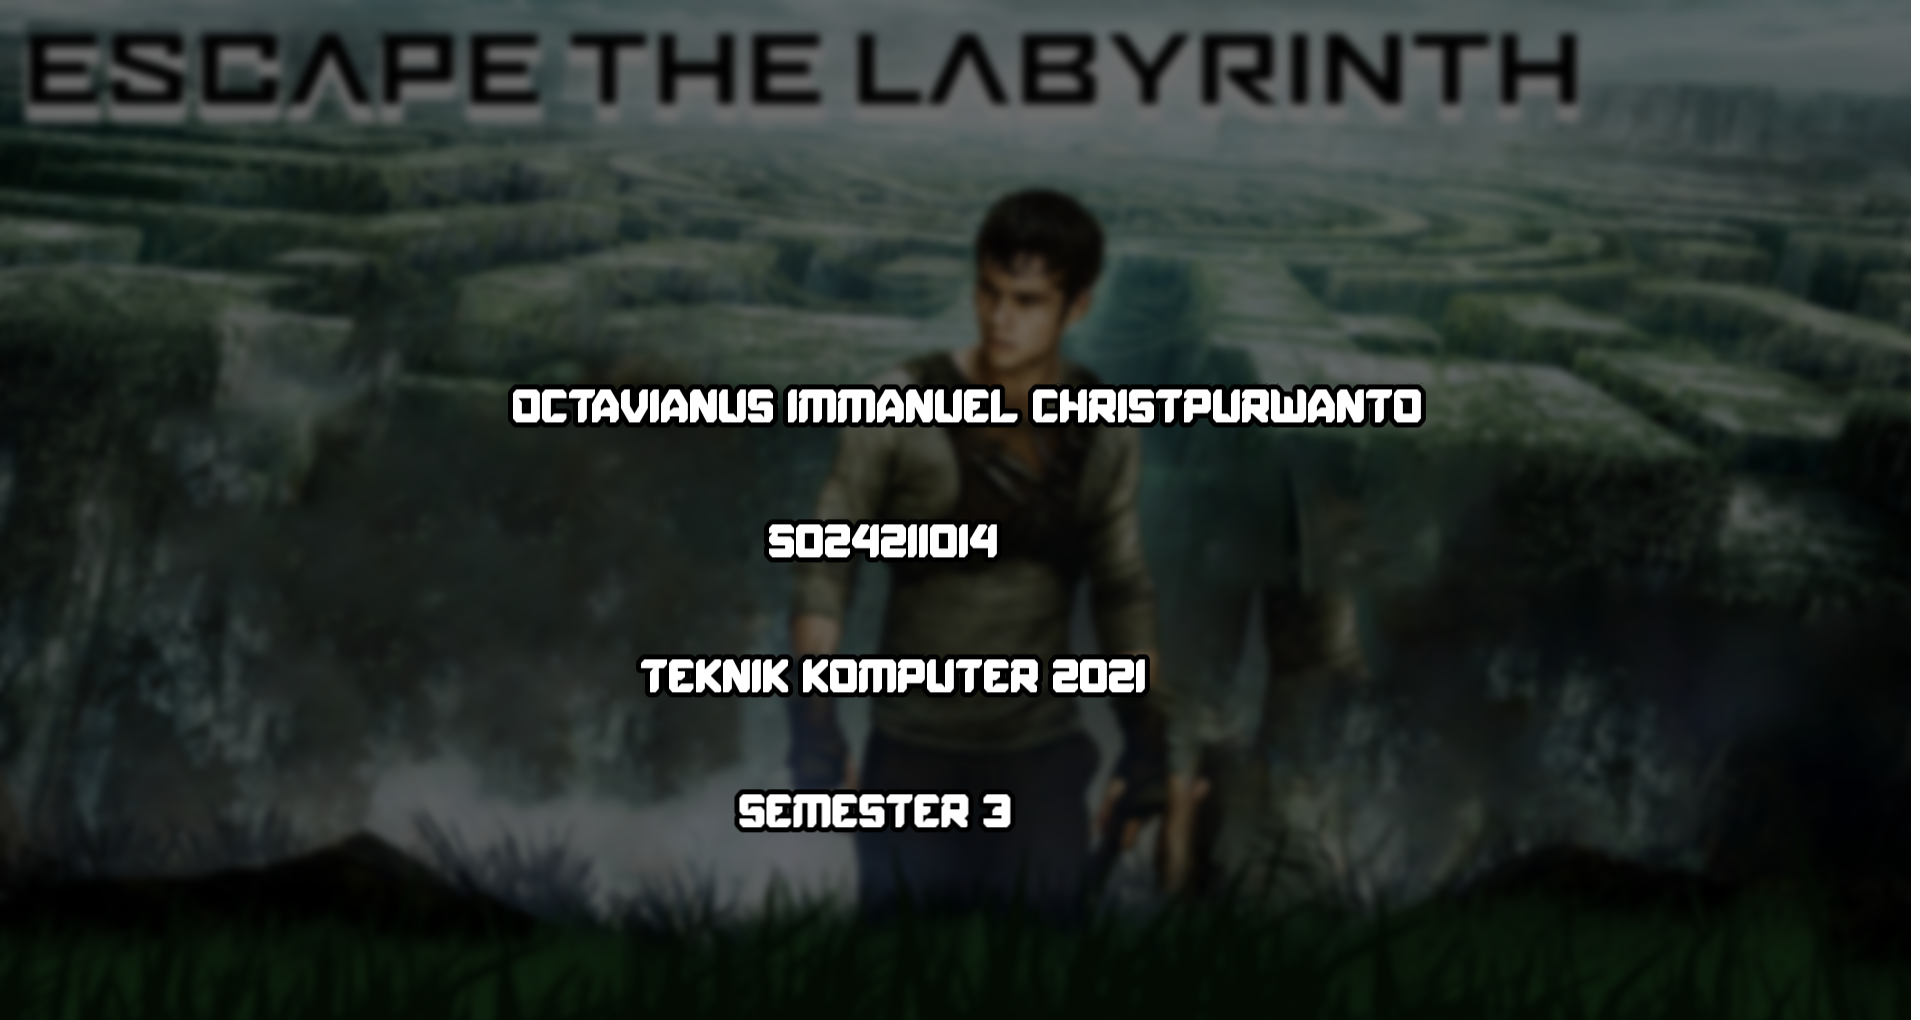
\includegraphics[width=10 cm]{Credits.png}
 		\caption{Credits}
 \end{figure}
 \begin{figure} [h]
 		\centering
 		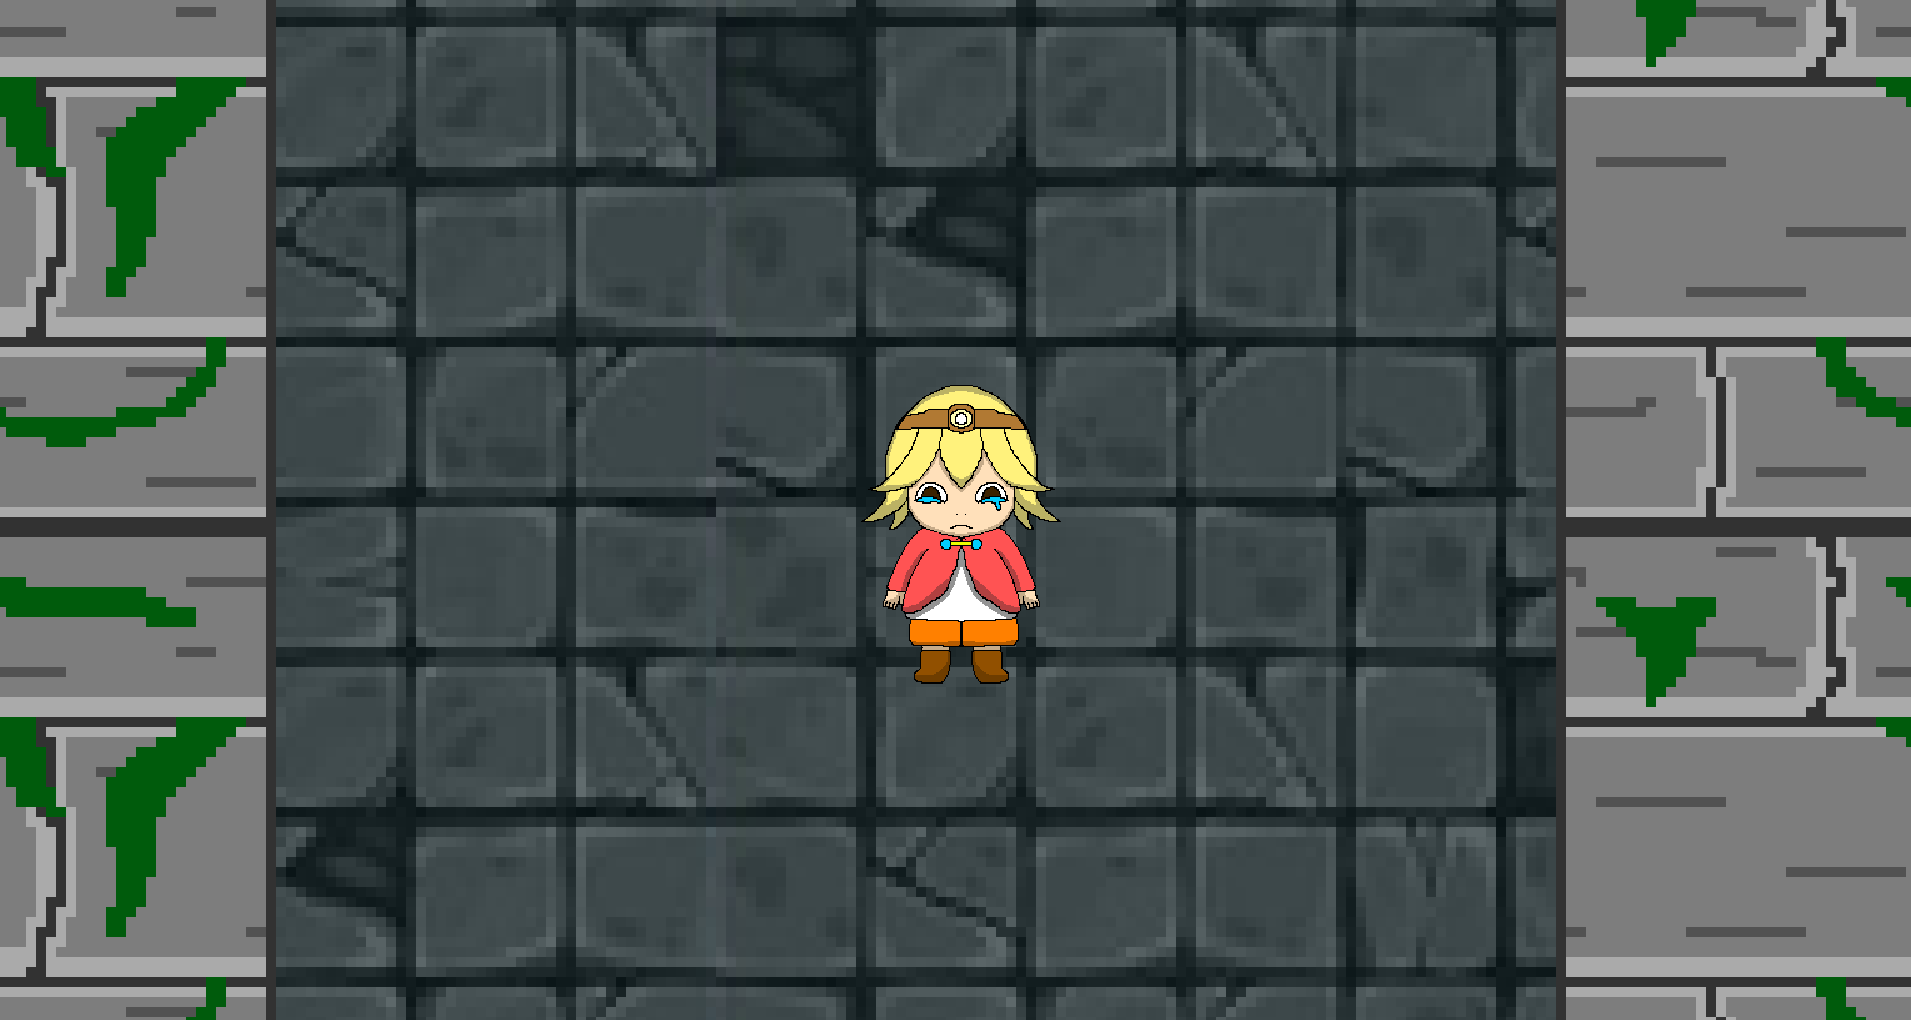
\includegraphics[width=10 cm]{Ingame.png}
 		\caption{Dalam Game}
\end{figure}
\begin{figure} [h]
\centering
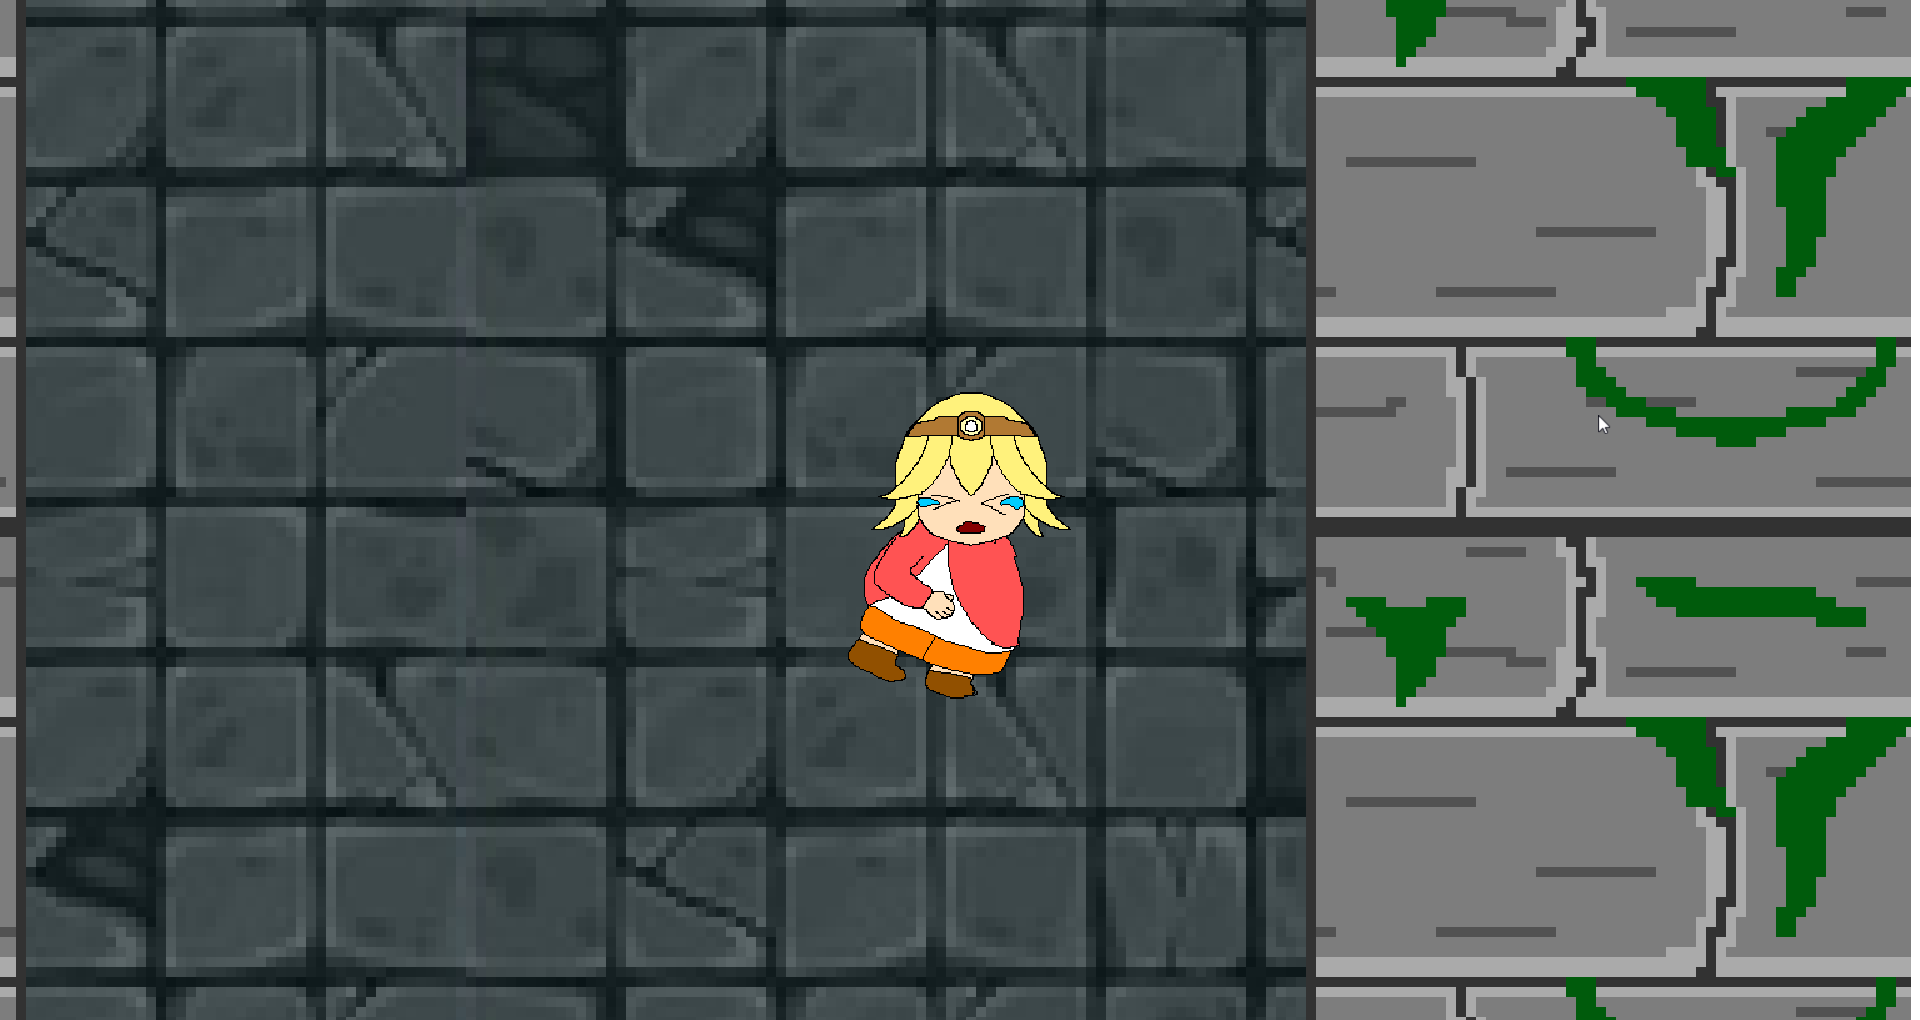
\includegraphics[width=10 cm]{Jalan Kanan.png}
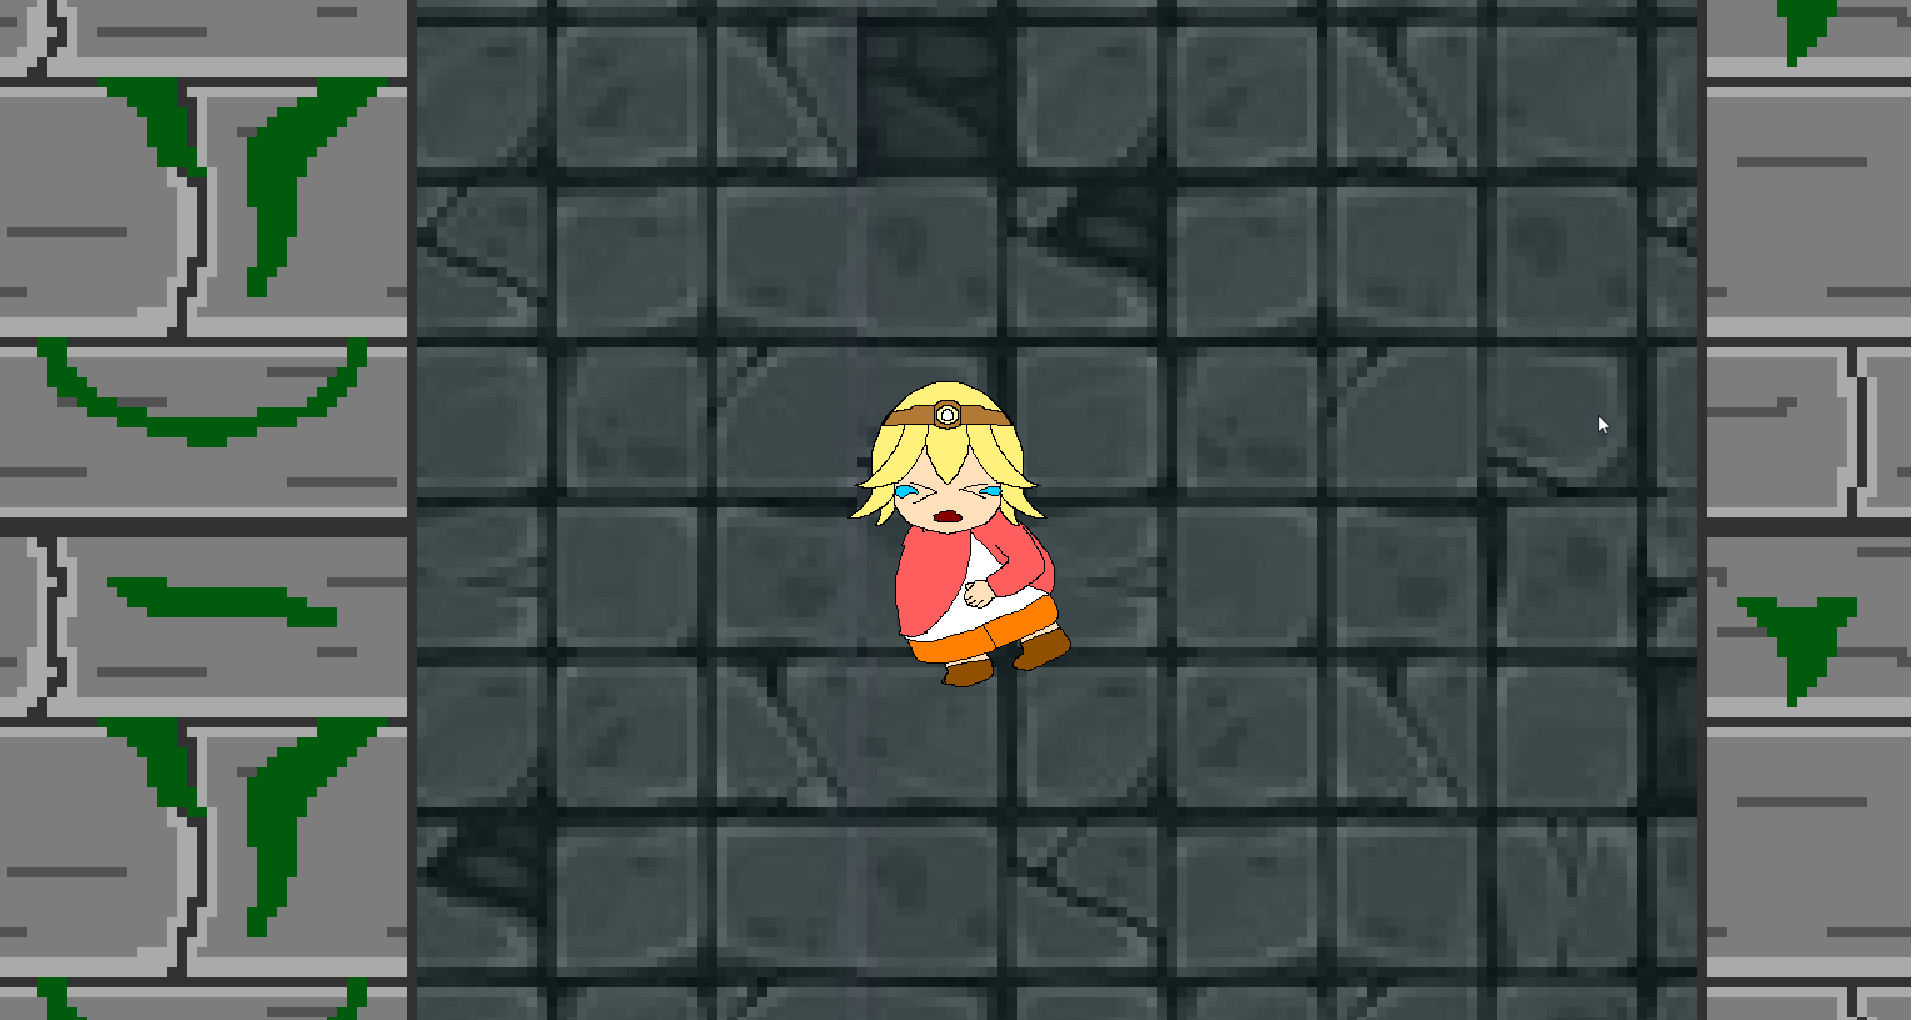
\includegraphics[width=10 cm]{Jalan Kiri.png}
\caption{Movement Karakter}
\end{figure}
\begin{figure} [h]
\centering
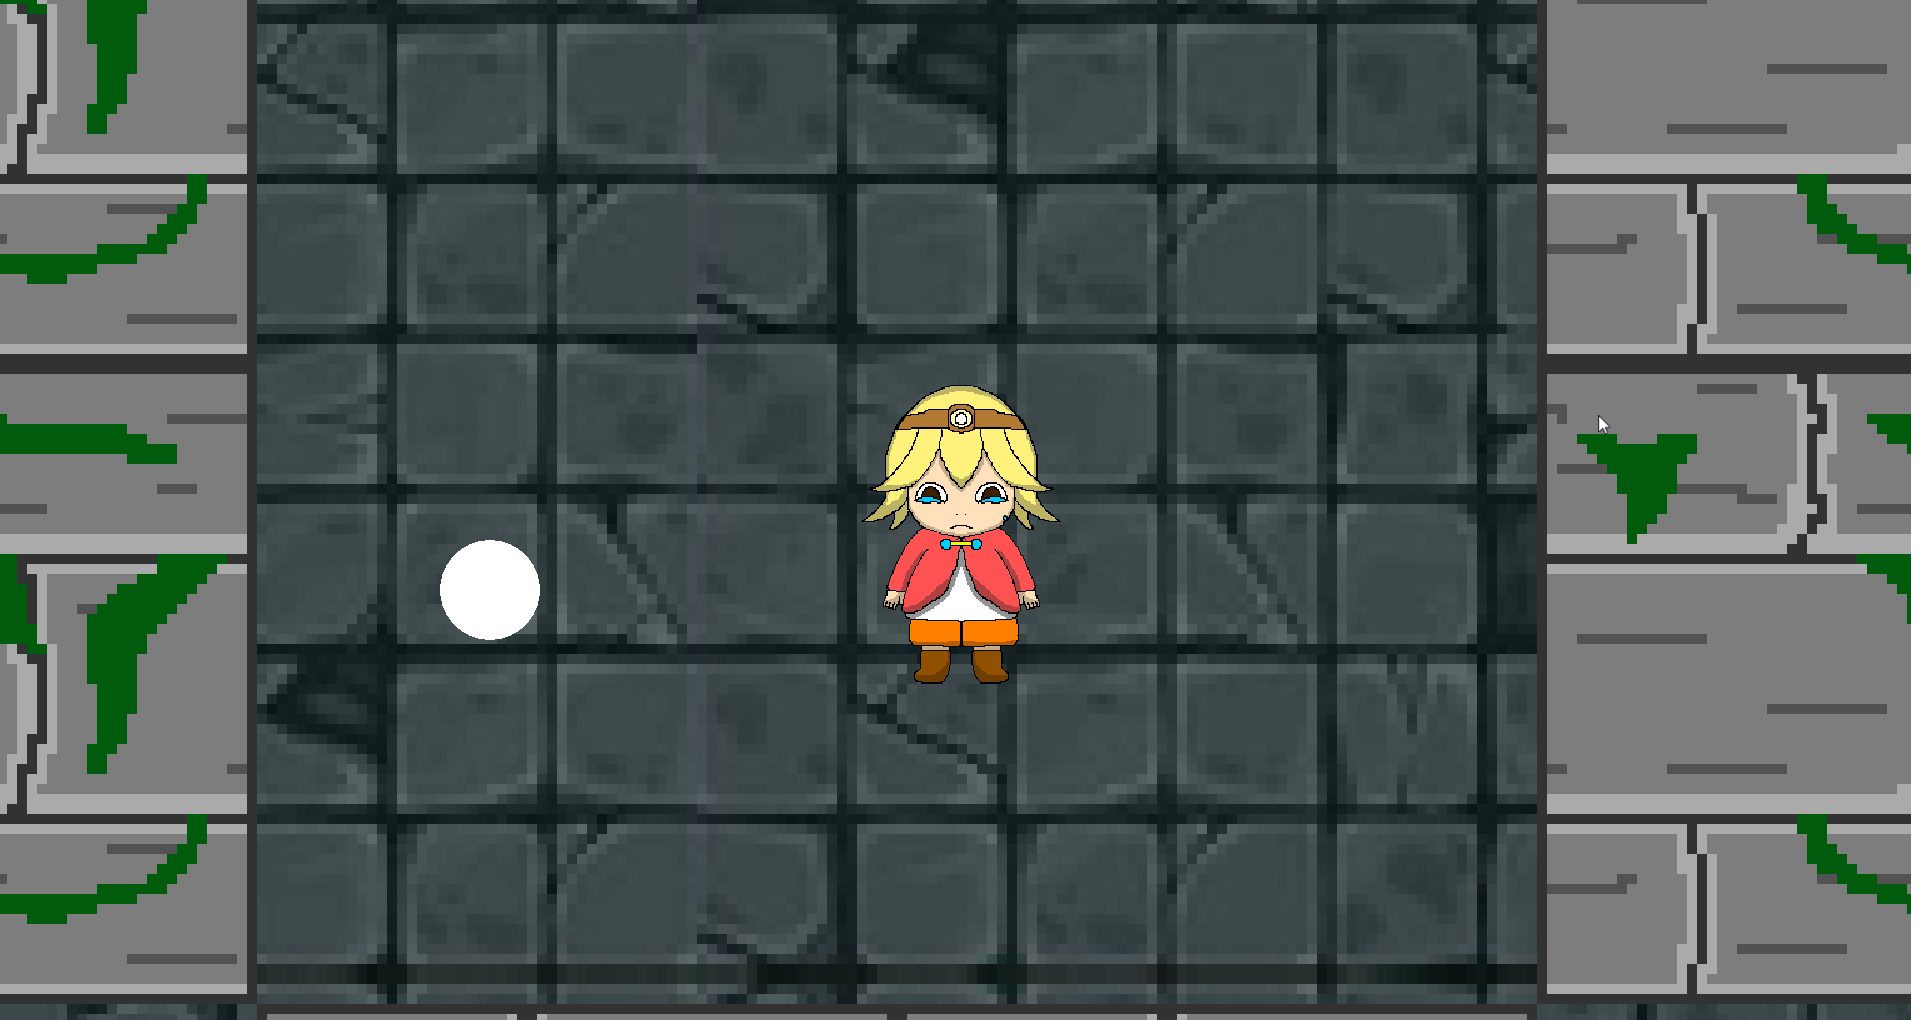
\includegraphics[width=10 cm]{Tembak.png}
\caption{Tembakan Peluru}
\end{figure}
\begin{figure} [h]
\centering
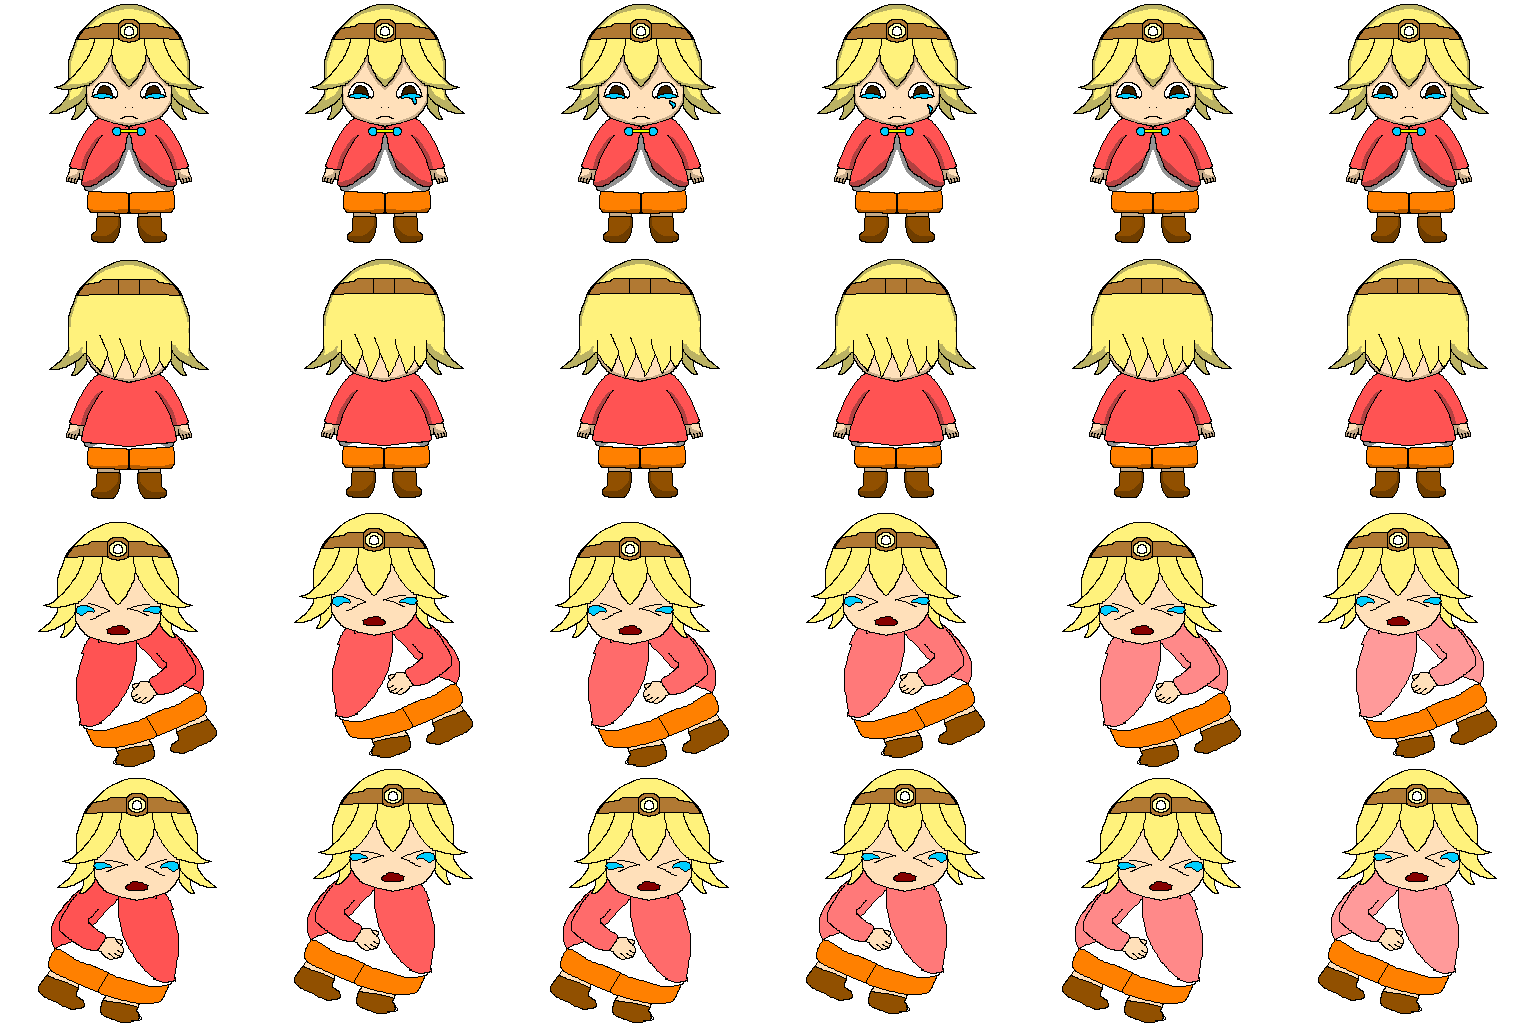
\includegraphics[width=10 cm]{CharacterSprite.png}
\caption{Animasi Karakter}
\end{figure}
\begin{figure} [h]
	\centering
	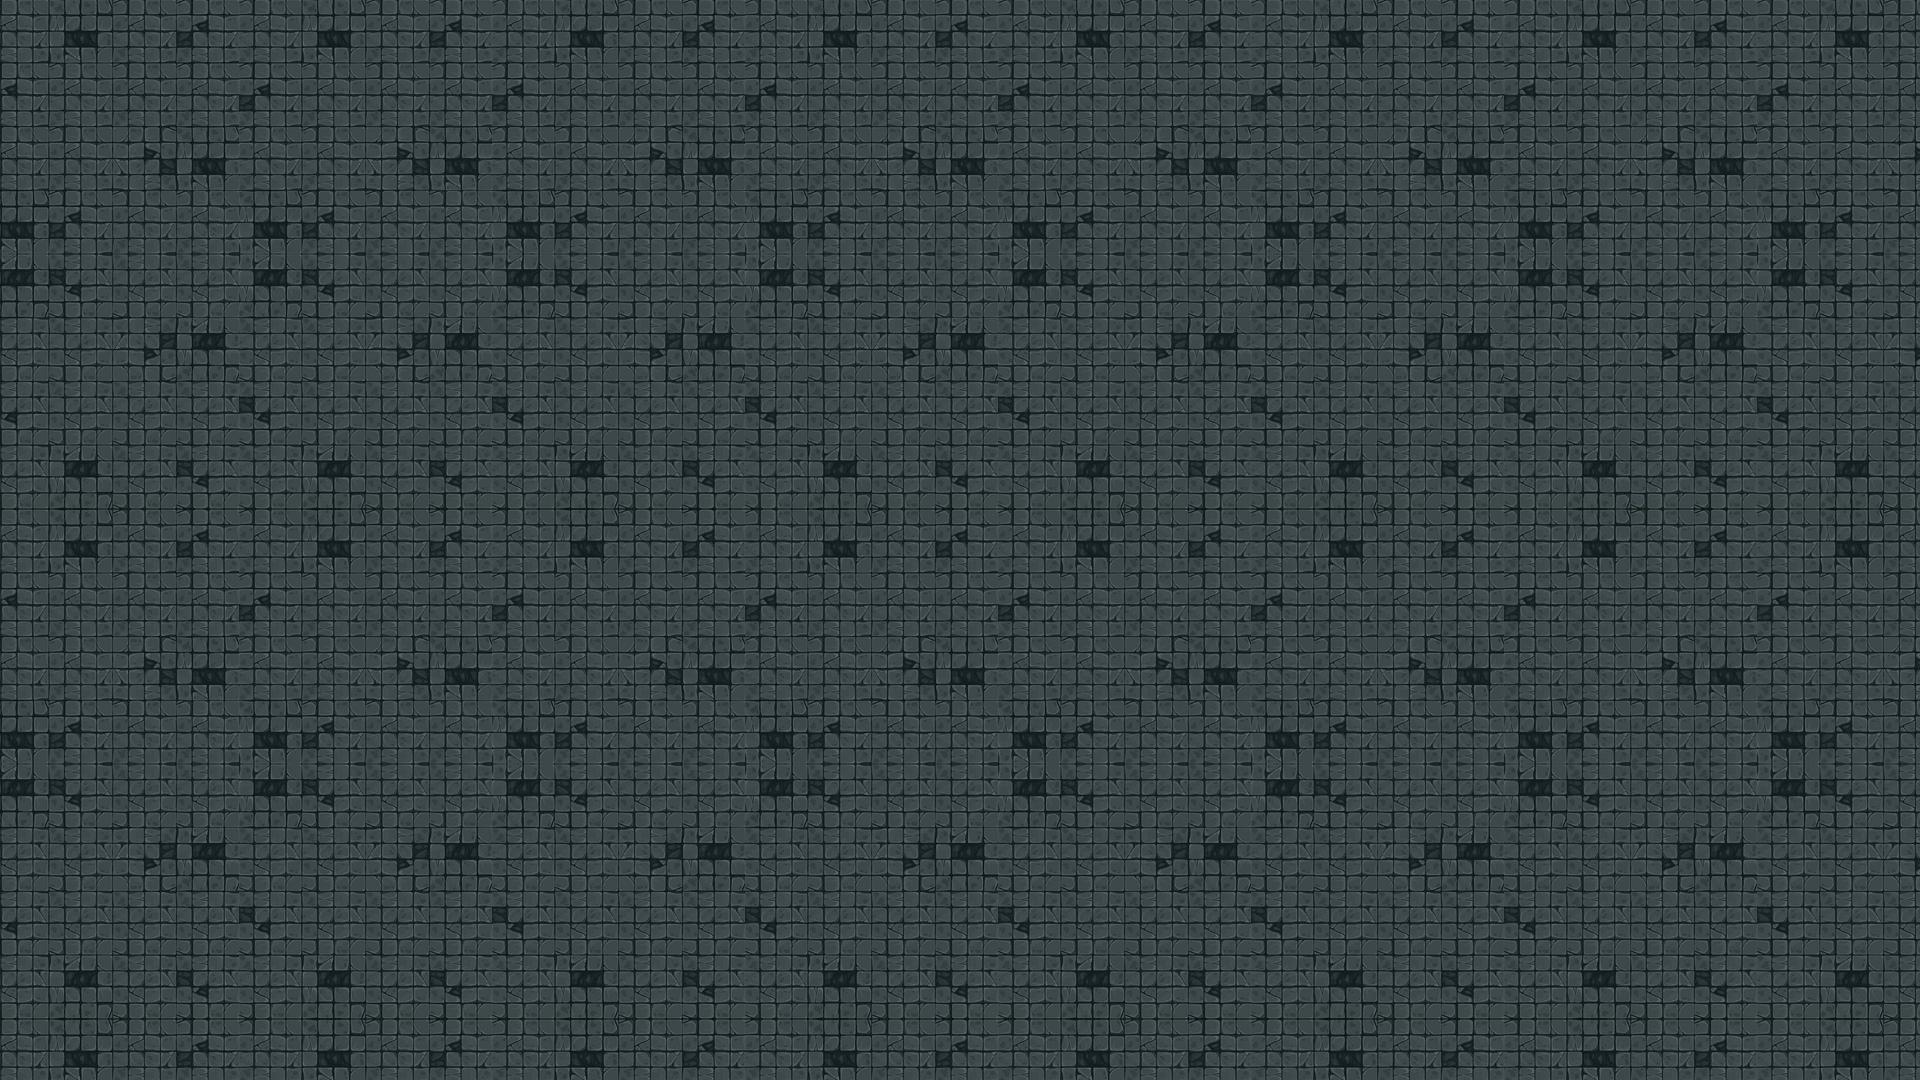
\includegraphics[width=10 cm]{Floor.png}
	\caption{Sprite Lantai}
\end{figure}
\begin{figure} [h]
	\centering
	
\includegraphics[width=8 cm]{Wall.png}
	\caption{Sprite Tembok}
\end{figure}

\chapter{Struktur Data Karakter}
\section{Codingan Player.h}

\begin{verbatim}
#ifndef PLAYER_H
#define PLAYER_H
#include "allinone.h"
#include "Animation.h"
#pragma once

using namespace sf;

class Peluru
{
	private:
	sf::Vector2f position;
	sf::Vector2f velocity;
	CircleShape shape;
	
	public:
	Peluru(sf::Vector2f position, sf::Vector2f velocity){
		shape = CircleShape(5);
		this->position = position;
		shape.setPosition(position);
		
		this->velocity = velocity;
	}
	
	void SetVelocity(sf::Vector2f val){ velocity = val; }
	void Update();
	CircleShape GetShape(){ return shape; }
	
};

class Player
{
	public:
	Player(sf::Texture* texture, sf::Vector2u imageCount, float switchTime, float speed);
	~Player();
	
	void Update(float deltaTime);
	void Draw(sf::RenderWindow& window);
	
	sf::Vector2f GetPosition() { return badan.getPosition();}
	void SetSpeed(float val){ speed = val; }
	void Tembak(Vector2f velocity);
	
	private:
	
	sf::RectangleShape badan; //untuk badannya
	Animation animasi; //untuk animasi saat jalan
	unsigned int row; //untuk row spritenya
	float speed;
	float initialSpeed;
	vector<Peluru> peluru;
	
	
	sf::SoundBuffer langkahsfxsb;
	sf::Sound langkahsfx;
	
	
};

#endif
\end{verbatim}
\section{Codingan Player.cpp}
\begin{verbatim}
	#include "Player.h"
	
	Player::Player(sf::Texture* texture, sf::Vector2u imageCount, float switchTime, float speed) :
	animasi(texture, imageCount, switchTime)
	{
		this->speed = speed;
		this->initialSpeed = speed;
		row = 0;
		
		badan.setSize(sf::Vector2f(32.0f, 32.0f));
		badan.setOrigin(badan.getSize() / 2.0f);
		badan.setPosition(500.0f, 500.0f);
		badan.setTexture(texture);
		
		if (!langkahsfxsb.loadFromFile("D:/Kebutuhan Game/_SFML/File Tambahan/walksfx.wav"))
		{
			std::cout << "SFX jalan error" << std::endl;
		}
		
		langkahsfx.setBuffer(langkahsfxsb);
		
	}
	
	Player::~Player()
	{
		
	}
	void Player::Update(float deltaTime) 
	{
		sf::Vector2f movement(0.0f, 0.0f);
		
		if (sf::Keyboard::isKeyPressed(sf::Keyboard::A))
		movement.x -= speed * deltaTime;
		if (sf::Keyboard::isKeyPressed(sf::Keyboard::D))
		movement.x += speed * deltaTime;
		if (sf::Keyboard::isKeyPressed(sf::Keyboard::W))
		movement.y -= speed * deltaTime;
		if (sf::Keyboard::isKeyPressed(sf::Keyboard::S))
		movement.y += speed * deltaTime;        
		
		if(movement.y == 0.0f)
		{
			row = 0;
		}
		else if (movement.y > 0.0f)
		{
			row = 1;
		}
		else 
		{
			row = 1;
		}
		
		if(movement.x == 0.0f)
		{
			row = 0;
		}
		else if (movement.x > 0.0f)
		{
			row = 3;
		}
		else
		{
			row = 2;
		}
		
		if (speed > initialSpeed) speed--;
		
		for(int i = 0; i < peluru.size(); i++){
			peluru[i].Update();
		}
		
		animasi.Update(row, deltaTime);
		badan.setTextureRect(animasi.uvRect);
		badan.move(movement);
	}
	
	void Player::Draw(sf::RenderWindow& window) 
	{
		window.draw(badan);
		for(int i = 0; i < peluru.size(); i++){
			window.draw(peluru[i].GetShape());
		}
	}
	
	void Player::Tembak(Vector2f velocity){
		Peluru p(this->GetPosition(), velocity);
		
		peluru.push_back(p);
	}
	
	void Peluru::Update(){    
		position += velocity;
		shape.setPosition(position);
	}
\end{verbatim}

\chapter{Struktur Penyimpanan Data dalam Memory}
Pada codingan \emph{game} saya ini, struktur penyimpanan data salah satunya terdapat pada bagian \emph{wallpaper background} menu utama. Contoh codingannya adalah sebagai berikut
\begin{verbatim}
	sf::RectangleShape background;
	sf::Texture texbackground;
	background.setSize(sf::Vector2f(1920,1080));
	texbackground.loadFromFile("File Tambahan/background.png");
	background.setTexture(&texbackground);
\end{verbatim}
Data \emph{wallpaper backgroundnya} yang nama filenya saya beri nama "background.png" disimpan di memori Texture pada sistem SFML yang memorinya saya beri nama "texbackground". Kemudian, saya membuat sebuah persegi yang saya beri nama "background" yang nantinya persegi tersebut akan saya ubah texturenya dengan file yang saya simpan di memori "texbackground" tadi. Saya set texture persegi "background" tadi dengan setTexture(texbackground), dengan demikian persegi tadi sekarang memiliki texture atau gambar sama dengan background yang tadi datanya kita simpan.
\chapter{Kesimpulan}
Kesimpulan yang saya dapat dari membuat game ini adalah bagaimana cara kita menyimpan suatu data yang akan kita gunakan nantinya, sehingga saat membutuhkan data tersebut tidak perlu repot-repot membuat data baru yang sama, tapi bisa dengan menyimpan data sebelumnya lalu jika ingin digunakan kita hanya perlu memanggil data tersebut. Game ini juga mengajarkan saya codingan karena pada awalnya saya memang tidak bisa coding sama sekali, sehingga dengan adanya tugas \emph{final project} pembuatan game ini, saya bisa belajar banyak.

\end{document}